\chapter{多无人机SLAM仿真} \label{Simulation}

% 介绍框架
本章主要多无人机SLAM的仿真;为了循序渐进,首先介绍仿真环境的配置,其次是单机的SLAM仿真,最后过渡到多机的SLAM仿真。


\section{gazebo仿真环境配置}

在进行仿真之前,首先要对场景进行搭建,对launch文件进行配置。

\subsection{场景} \label{4.1.1}

仿真环境中,场景的设计不能过于简单,墙壁、地面等大面积重复物体应该具有纹理,否则ORB-SLAM2的特征点提取会十分困难;除了纹理的设计,还应尽可能多地提供物体,使场景丰富。如图\ref{fig3-1}所示:

\begin{figure}[!ht]
	\centering
	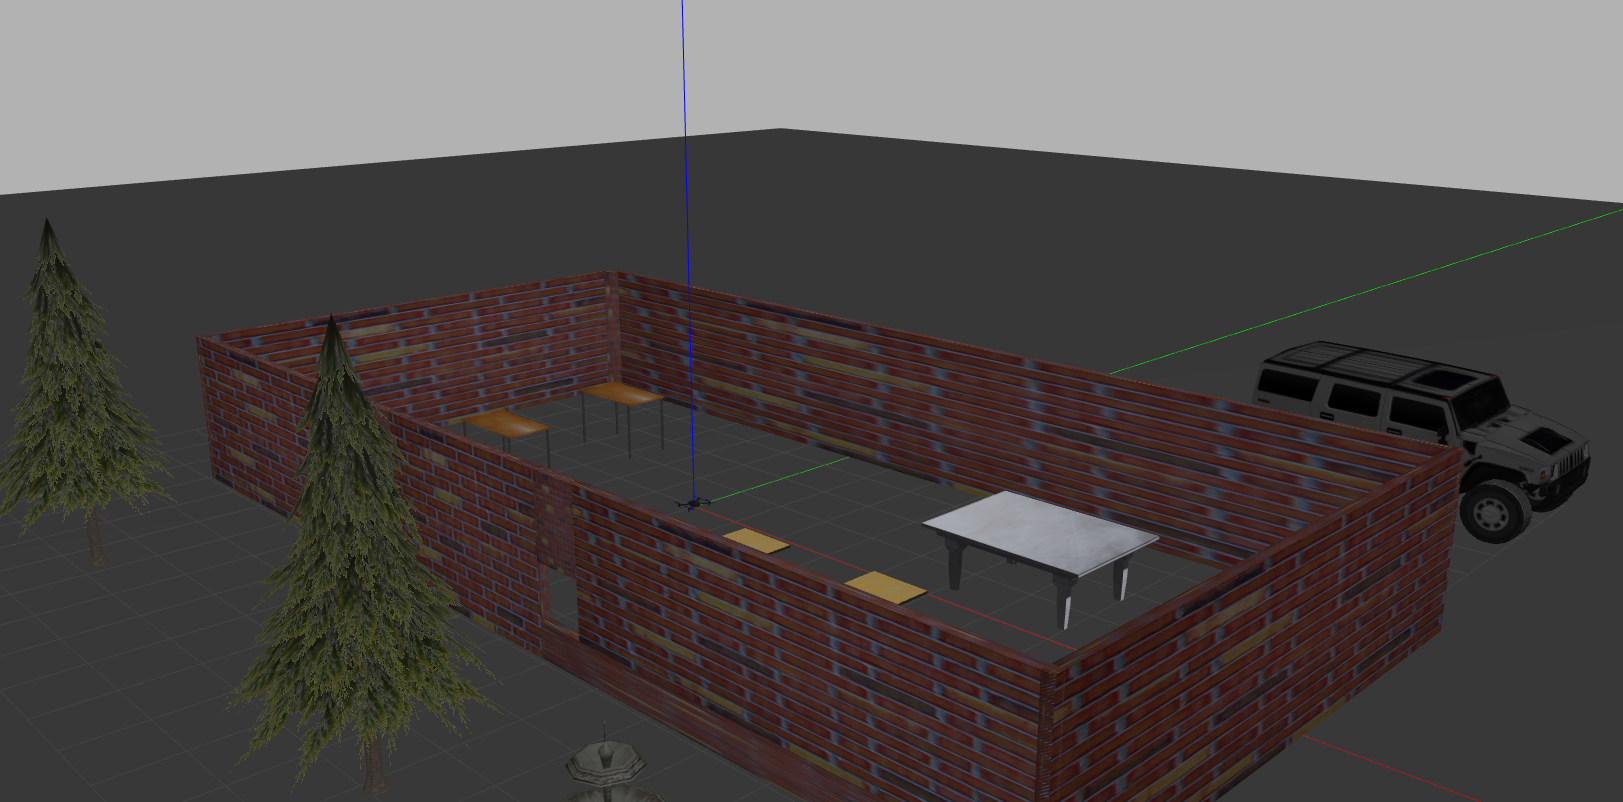
\includegraphics[width=0.7\textwidth]{scene.png}
	\caption{gazebo场景示例}
	\label{fig4-1}
\end{figure}

进入gazebo界面后,使用Control+B进入其编辑界面;之后有两种选择:

\begin{enumerate}
	\item 建立基础模型,一般在这里会绘制上地面及其纹理;如果是室内场景,还会绘制一个大致的墙壁结构,墙壁的纹理,其上的门窗等;最后将该模型保存到.gazebo/model文件中,这是gazebo模型的默认文件。
	\item 直接选择插入模型;可以在此直接插入上文建立的基础模型,也可以插入其他模型库已有的模型,默认存储在/.gazebo/models文件夹下
\end{enumerate}

最后需要将自建场景存储为一个.world文件,gazebo不会给文件后缀的提示,需要自己输入后缀,这一点需要特别注意。在此之后,就获得了自建的world场景,下一步需要在launch文件中更改该项,完成调用。


\subsection{launch文件} \label{4.1.2}

\ref{2.1.2}节中,曾简单介绍launch文件的功能。作为整个仿真环境的配置文件,launch文件中基本包含了仿真所需的参数。

launch文件使用XML标签语言书写,主要为确定启动的节点和加载参数使用,简单的开始节点、加载参数的方法如下:

\begin{lstlisting}[language={XML}]
<node pkg="your package name" name="your node name" type="your node type"/>
<param name="param name" value="param value"/>
<arg name="arg name" default="arg value"/>
\end{lstlisting}

在一个简单的launch文件中,主要会包括设备的信息设置、PX4配置和gazebo仿真配置。

\begin{enumerate}
	\item 设备的信息设置;这一部分包括设备的位姿,通过$x,y,z,R,P,Y$6个变量表示三维位置坐标和滚转、俯仰、偏航姿态角;还包括设置设备的类型和名称,在四旋翼无人机仿真中使用iris作为参数vehicle的值,并且在sdf参数中,将sdf参数的值指向iris的sdf文件(一般在该位置,都使用默认参数加find指令去寻找软件在环仿真的gazebo模型路径);最后是一些gui等参数的设置,默认使用官方设置的即可。
	\item PX4软件在环仿真的参数;在这里启动了名为sitl的节点,其参数指向了EKF设置的rcS文件;
	\item gazebo仿真参数配置;在这里需要修改world\_name参数,其默认是world参数的值,所以实际上也可以直接修改world参数值,将其指向自建的world文件。
\end{enumerate}

自此,launch文件配置完成,可以使用PX4启动launch文件来进行简单的仿真。


\section{单机SLAM仿真}

在进行多机仿真前,首先要进行单机的SLAM仿真,为多机仿真做铺垫。单机SLAM仿真分为单机Offboard模式起降和航路点飞行,以及SLAM下的起降和航路点飞行四步。

\subsection{launch文件配置} \label{4.2.1}

\ref{4.1.2}节中介绍了launch文件的详细配置方法,对于单机的SLAM仿真,配置方法基本与其相同,但是需要给iris无人机假装上双目相机。以下介绍给无人机加装相机的方法:

选择mavros\_posix\_sitl.launch文件,找到设备模型和世界配置区块,原始设置如下:

\begin{lstlisting}[language={XML}]
<!-- vehicle model and world -->
<arg name="est" default="ekf2"/>
<arg name="vehicle" default="iris"/>
<arg name="world" default="$(find mavlink_sitl_gazebo)/worlds/empty.world"/>
<arg name="sdf" default="$(find mavlink_sitl_gazebo)/models/$(arg vehicle)/$(arg vehicle).sdf"/>
\end{lstlisting}

加载双目相机,也就是给iris无人机装上相机,需要在设备配置处,加上其附加配置的sdf文件;由于在这里只添加了相机的sdf文件,所以该附加sdf文件不需要手动修改,直接链接到相机上即可。因此需要新建camera参数,其值为iris\_stereo\_camera,是gazebo自带的可以添加到iris无人机上的双目相机,修改后的launch文件部分如下:

\begin{lstlisting}[language={XML}]
<!-- vehicle model and world -->
<arg name="est" default="ekf2"/>
<arg name="vehicle" default="iris"/>
<!-- add stereo camera for iris -->
<arg name="my_camera" default="iris_stereo_camera"/>
<arg name="world" default="$(find mavlink_sitl_gazebo)/worlds/empty.world"/>
<!-- also need to revise sdf -->
<arg name="sdf" default="$(find mavlink_sitl_gazebo)/models/$(arg my_camera)/$(arg my_camera).sdf"/>
<!-- <arg name="sdf" default="$(find mavlink_sitl_gazebo)/models/$(arg vehicle)/$(arg vehicle).sdf"/> -->
\end{lstlisting}

更改完launch文件的无人机配置后,可以试运行来检测,即roslaunch该launch文件。之后有两种方法可以检查,一是使用rostopic list命令,查找当前活跃的话题,如果MAVROS能顺利连接上双目相机,则会出现image\_raw话题(对于双目分为左右,但对于单目仅有一个话题),这种情况下一般是成功的;另一种方法是使用ROS自带的rqt\_graph命令,该命令可以以图的形式展示出,这种方式用途更广。装配成功后,仿真加载时应如图\ref{fig4-2}所示:

% 或许可以加一张大图

\begin{figure}[!ht]
	\centering
	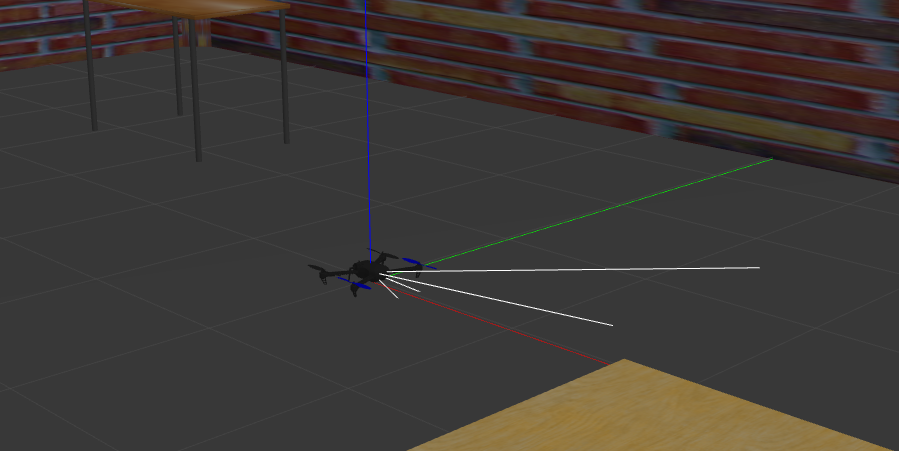
\includegraphics[width=0.7\textwidth]{mono_uav.png}
	\caption{装配相机的iris无人机}
	\label{fig4-2}
\end{figure}

需要注意,在需要与MAVROS建立通信的launch文件中,需要设置fcu端口号,具体表示为udp+本地端口号,在多机的launch文件中,每一架飞机的端口号都是不同的,但单机不需要作出修改。

如果设置双目相机参数后加载失败或加载到一个正方体模型,则是双目相机模型缺失导致的。一种方法是删除gazebo自带的models中的双目相机,并用PX4中的双目相机模型代替;另一种方法则是直接将sdf的值指向PX4的双目相机,即其值为PX4双目相机的路径。

\subsection{Offboard程序} \label{4.2.2}

完成双目相机的配置后,第二步是进入Offboard程序。与\ref{2.2.3}的Offboard模式类似,首先目标是完成一套完整的起飞降落。需要注意,Offboard模式中,所有消息指令都需要以大于$2Hz$的频率发送,否则会激活安全生效机制,飞机返航。

\begin{enumerate}
	\item 起飞的方式。动力学模型上的起飞即给四旋翼增加动力,保持平衡并提供向上的大于重力的升力,在程序中表示为发布位置指令,该消息类型为MAVROS的geometry\_msgs数据类型。
	\item 降落的方式。一般使用切换飞行模式的方法,将飞行模式切换到降落模式,选择降落模式中的自动降落即可。
\end{enumerate}

降落的程序如下:

\begin{lstlisting}[language={C++}]
// proceed landing process
ROS_INFO("landing");
mavros_msgs::SetMode land_set_mode;
land_set_mode.request.custom_mode = "AUTO.LAND";
while (ros::ok()){
if( current_state.mode != "AUTO.LAND" &&
(ros::Time::now() - last_request > ros::Duration(5.0))){
if( set_mode_client.call(land_set_mode) &&
land_set_mode.response.mode_sent){
ROS_INFO("Land enabled");
}
last_request = ros::Time::now();
}
if(!current_state.armed){
break;
}

ros::spinOnce();
rate.sleep();
}
\end{lstlisting}

航路点飞行的简单实现方法为,依次发布各航路点的位置信息,但需要一个函数去判断飞机是否到达了航路点。函数的实现可以利用预计坐标和现处位置之间的欧式距离作评判标准,小于某值则认为到达航路点,实现的关键在现处位置消息的订阅。首先需要定义current\_pose作为现处位置的变量,之后定义回调函数,获得该信息,实现的代码如下:

\begin{lstlisting}[language={C++}]
// record current pose
geometry_msgs::PoseStamped current_pose; /* NOLINT */

// callback function for Subscriber for local_pos_sub
void local_cb(const geometry_msgs::PoseStamped::ConstPtr& msg){
current_pose = *msg;
}
\end{lstlisting}

检查是否到达航路点的函数如下:

\begin{lstlisting}[language={C++}]
// check if reached a waypoint
bool check_waypoint(const geometry_msgs::PoseStamped &now_pose, const geometry_msgs::PoseStamped &aim_pose){
// define Point to hold current position and aim position
geometry_msgs::Point curr, aim;
curr = now_pose.pose.position;
aim = aim_pose.pose.position;
double precision = 0.1;

// define return value
bool reach = false;

// calculate distance
double dist = sqrt(pow((curr.x - aim.x), 2) +
pow((curr.y - aim.y), 2) + pow((curr.z - aim.z), 2));
if(dist < precision){
reach = true;
ROS_INFO("reached waypoint!");
}

return reach;
}
\end{lstlisting}

前往下一个航路点的方法如下:

\begin{lstlisting}[language={C++}]
// set second waypoint
geometry_msgs::PoseStamped pose2;
pose2.pose.position.x = 2;
pose2.pose.position.y = 2;
pose2.pose.position.z = 2;

// heading for waypoint 2
while(ros::ok()){
// publish pose1 information
local_pos_pub.publish(pose2);
ros::spinOnce();

// check if reached a waypoint
if (check_waypoint(current_pose, pose2)) break;
rate.sleep();
}
\end{lstlisting}

按2个航路点飞行的地面站轨迹示意图如图\ref{fig4-3}所示:

\begin{figure}[!ht]
	\centering
	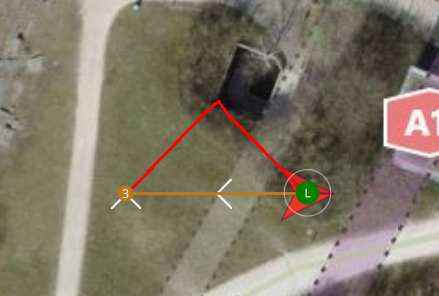
\includegraphics[width=0.6\textwidth]{waypoint.png}
	\caption{地面站的航路点飞行轨迹}
	\label{fig4-3}
\end{figure}

\subsection{视觉定位的坐标变换} \label{4.2.3}

在正常GPS定位的Offboard模式下,飞机的位置在MAVROS中作为已知量存在。但在视觉定位模式下,MAVROS需要通过vision\_pose/pose话题获得飞机的位姿信息。而ORB-SLAM2解算出的位姿并不是MAVROS的地理位置消息格式,因此需要做一些转换。

\begin{figure}[!ht]
	\centering
	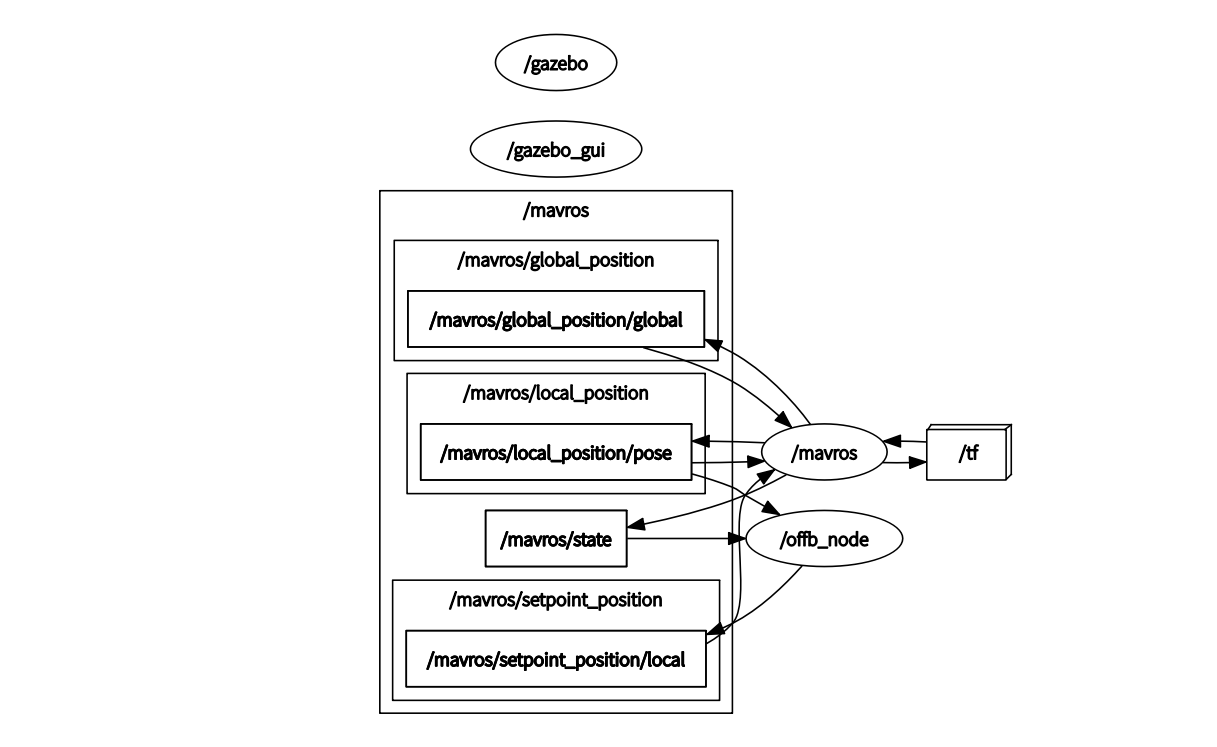
\includegraphics[width=0.8\textwidth]{rqtOffboard.png}
	\caption{Offboard节点话题关系}
	\label{fig4-4}
\end{figure}

\begin{figure}[!ht]
	\centering
	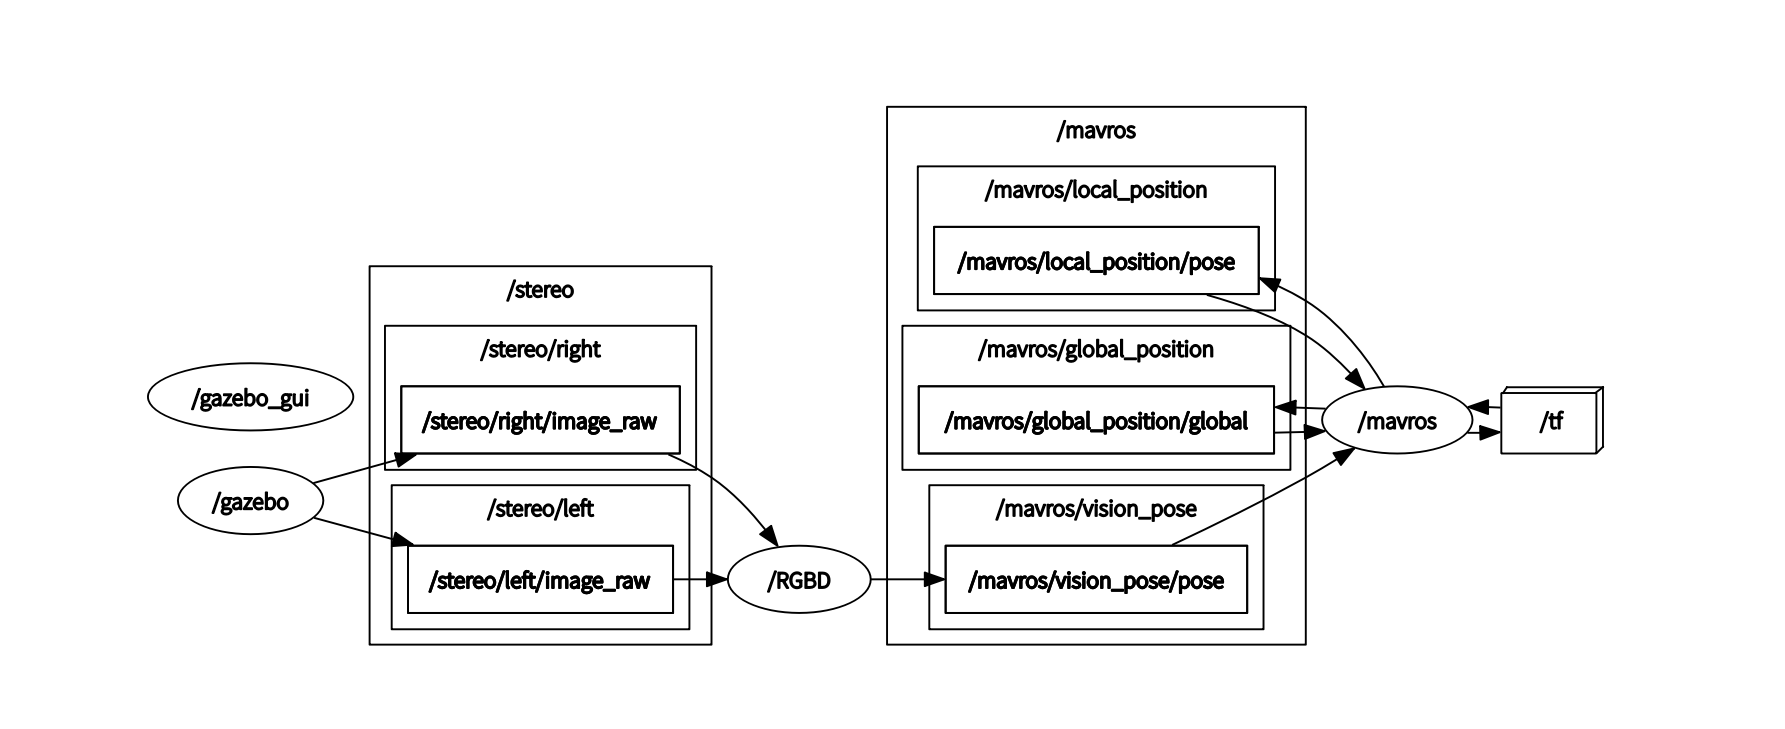
\includegraphics[width=0.4\textwidth]{rqtRGBD.png}
	\caption{视觉SLAM节点话题关系}
	\label{fig4-5}
\end{figure}

ORB-SLAM2得到的外参$\bf{Tcw}$矩阵为$4 \times 4$矩阵:

$$
\bf{Tcw}=\begin{bmatrix}
\bf{R_{cw}} & \bf{t_{cw}}\\0 & 1
\end{bmatrix}
$$
其中,$\bf{R_{cw}}$为旋转矩阵,$\bf{t_{cw}}$为平移向量。

可以证明,从相机的外参矩阵得到相机位姿:

$$
\begin{aligned}
\bf{R_{wc}}= &\bf{R_{cw}}^T\\
\bf{t_{wc}}= &-\bf{R_{wc}} \cdot  \bf{t_{cw}}
\end{aligned}
$$

在此之后,还需要将$\bf{R_{wc}}$和$\bf{t_{wc}}$赋值给ROS中tf坐标系类型的Transform变量,之后通过调用ROS的poseTFToMsg函数,将tf类型的变量转为MAVROS的地理位置消息类型变量。实现的代码如下:

\begin{lstlisting}[language={C++}]
Rwc = Tcw.rowRange(0,3).colRange(0,3).t(); // Rotation information
twc = -Rwc*Tcw.rowRange(0,3).col(3); // translation information
vector<float> q = ORB_SLAM2::Converter::toQuaternion(Rwc);

tf::Transform new_transform;
new_transform.setOrigin(tf::Vector3(twc.at<float>(0, 0), twc.at<float>(0, 1), twc.at<float>(0, 2)));

tf::Quaternion quaternion(q[0], q[1], q[2], q[3]);
new_transform.setRotation(quaternion);

tf::poseTFToMsg(new_transform, pose.pose);
x = pose.pose.position.x;
y = pose.pose.position.y;
z = pose.pose.position.z;
pose.pose.position.x = z;
pose.pose.position.y = -x;
pose.pose.position.z = -y;
orb_pub->publish(pose);
\end{lstlisting}

\subsection{单机仿真实验结果} \label{4.2.4}

% 多补充几张图

进行起飞后SLAM建图的结果:

\begin{figure}[!ht]
	\centering
	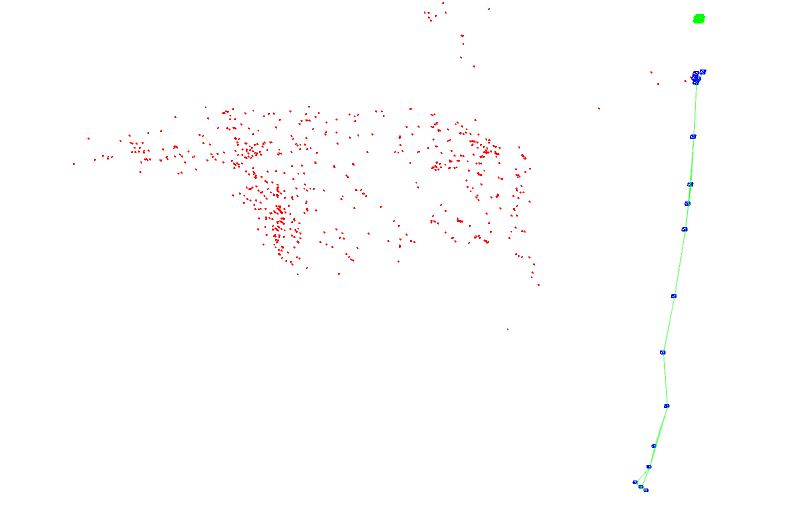
\includegraphics[width=0.4\textwidth]{single.png}
	\caption{单机SLAM的效果}
	\label{fig4-6}
\end{figure}




\section{多机SLAM仿真}


\subsection{launch文件配置} \label{4.3.1}

多机配置与单机配置最大的区别是,引用的子文件不同;单机引用posix\_sitl文件,而多机则引用vehicle\_spawn文件,而spawn文件是多机所独有的。

进入多机的launch文件,则需要引入组的概念。一个组使用一个命名空间,具有一套MAVROS的配置信息,多个组可以并行存在。因此在多机的launch文件设计中,一个组就是一架飞机,需要设置该组的命名空间,该组下的所有话题将共同使用该命名空间开头的话题。除此之外,还需要修改无人机的ID,ID默认从0到10;之后修改fcu地址和MAVLINK的udp端口,一般在末尾加上该无人机的ID即可。完整的双机launch配置代码如下:

\begin{lstlisting}[language={XML}]
<!-- UAV0 -->
<group ns="uav0">
<!-- MAVROS and vehicle configs -->
<arg name="ID" value="0"/>
<arg name="fcu_url" default="udp://:14540@localhost:14580"/>
<!-- PX4 SITL and vehicle spawn -->
<include file="$(find px4)/launch/single_vehicle_spawn_rcs.launch">
<arg name="x" value="0"/>
<arg name="y" value="0"/>
<arg name="z" value="0"/>
<arg name="R" value="0"/>
<arg name="P" value="0"/>
<arg name="Y" value="0"/>
<arg name="vehicle" value="$(arg vehicle)"/>

<arg name="my_camera" value="iris_fpv_cam"/>

<arg name="mavlink_udp_port" value="14560"/>
<arg name="mavlink_tcp_port" value="4560"/>
<arg name="ID" value="$(arg ID)"/>
<arg name="gst_udp_port" value="$(eval 5600 + arg('ID'))"/>
<arg name="video_uri" value="$(eval 5600 + arg('ID'))"/>
<arg name="mavlink_cam_udp_port" value="$(eval 14530 + arg('ID'))"/>


</include>
<!-- MAVROS -->
<include file="$(find mavros)/launch/px4.launch">
<arg name="fcu_url" value="$(arg fcu_url)"/>
<arg name="gcs_url" value=""/>
<arg name="tgt_system" value="$(eval 1 + arg('ID'))"/>
<arg name="tgt_component" value="1"/>
</include>
</group>

<!-- UAV1 -->
<group ns="uav1">                              
<!-- MAVROS and vehicle configs -->
<arg name="ID" value="1"/>
<arg name="fcu_url" default="udp://:14541@localhost:14581"/>
<!-- PX4 SITL and vehicle spawn -->
<include file="$(find px4)/launch/single_vehicle_spawn_rcs.launch">
<arg name="x" value="2"/>
<arg name="y" value="0"/>
<arg name="z" value="0"/>
<arg name="R" value="0"/>
<arg name="P" value="0"/>
<arg name="Y" value="0"/>
<arg name="vehicle" value="$(arg vehicle)"/>

<arg name="my_camera" value="iris_fpv_cam"/>

<arg name="mavlink_udp_port" value="14561"/>
<arg name="mavlink_tcp_port" value="4560"/>
<arg name="ID" value="$(arg ID)"/>
<arg name="gst_udp_port" value="$(eval 5600 + arg('ID'))"/>
<arg name="video_uri" value="$(eval 5600 + arg('ID'))"/>
<arg name="mavlink_cam_udp_port" value="$(eval 14530 + arg('ID'))"/>


</include>
<!-- MAVROS -->
<include file="$(find mavros)/launch/px4.launch">
<arg name="fcu_url" value="$(arg fcu_url)"/>
<arg name="gcs_url" value=""/>
<arg name="tgt_system" value="$(eval 1 + arg('ID'))"/>
<arg name="tgt_component" value="1"/>
</include>
</group>
\end{lstlisting}

其默认每架无人机调用的是spawn文件,其中关键的模型组合有两种方式,一种是使用urdf进行模型配置,一种是使用新的sdf。具体使用哪种视PX4的版本而定,由于urdf模型的配制方法要旧于sdf,新版的PX4统一使用sdf进行gazebo仿真的模型配置,并且使用jinja.py脚本生成sdf模型配置。

\begin{figure}[!ht]
	\centering
	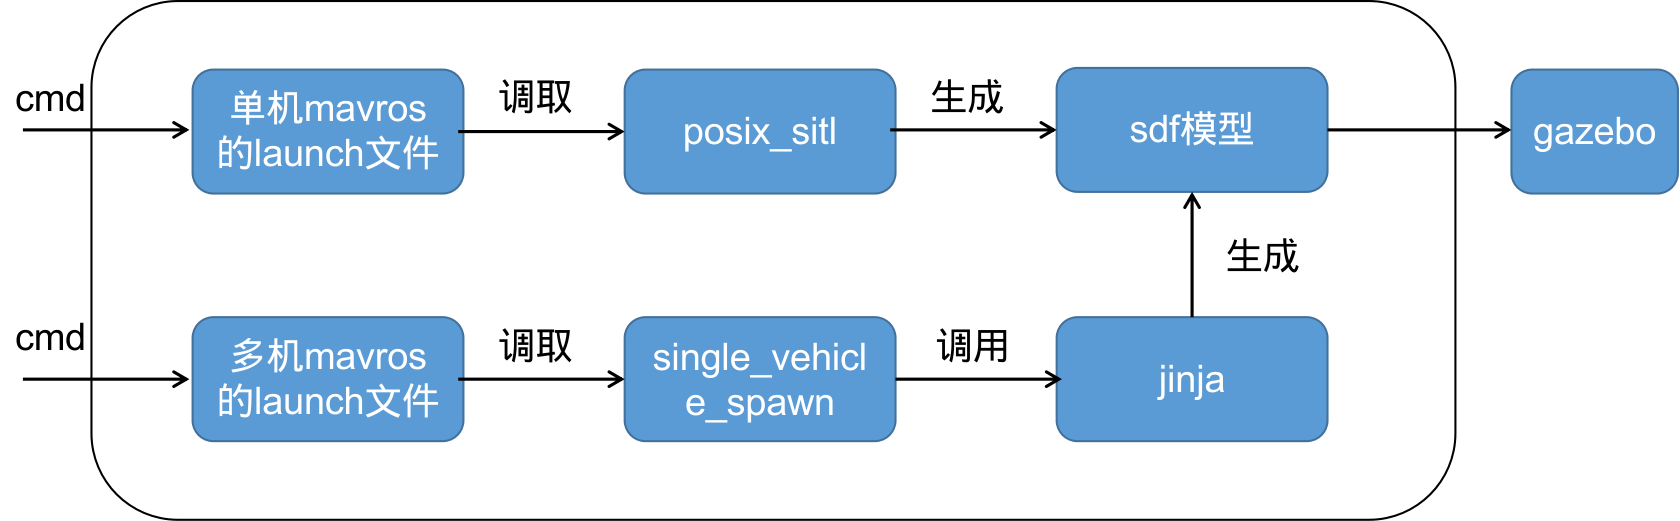
\includegraphics[width=0.8\textwidth]{sdf.png}
	\caption{仿真模型生成流程}
	\label{fig-sdf}
\end{figure}

图\ref{fig-sdf}展示了PX4中使用gazebo生成模型的方法,决定了修改模型的方法。可以看出,launch文件分为顶层和底层文件;平常直接使用roslaunch命令启动的一般为顶层文件,而顶层文件中调取的一般为底层文件。对于单机和多机,其调用的底层文件不同;单机调取posix\_sitl.launch文件,而多机则调取single\_vehicle\_spawn文件。二者的区别是单机的底层文件直接使用了即有的sdf模型,但多机的底层文件基于spawn繁殖机制,重新调用jinja生成了新的sdf模型,并且在该过程中对MAVLINK的许多参数作了配置,这一点是单机所没有的。最终都生成gazebo可以加载出的模型文件。

旧版本使用urdf版本的PX4,如果在launch文件中直接将其修改为sdf格式生成的模型,一般会报错jinja.py文件中有很多参数未定义,一种简单的处理方式是直接将新版本的janja替换到旧版本中去(为什么要使用旧版本,因为新版本的稳定性可能存在一些问题),但是这样做可能会连带产生一些附加问题,尽量选择不修改jinja这种较为底层的文件。

由于ROS的机制,话题如果重复,则会报错,并用时间戳最新的话题替换掉时间戳更旧的话题;如果多架无人机的话题不加以区分,可能会导致最终话题重复,从而只有一架无人机可以使用。


\subsection{多机编队处理} \label{4.3.2}

多机的控制可以使用编队控制,控制方法可以分为两种:集中式和分布式。

\begin{enumerate}
	\item 集中式即集群中存在领机,其他飞机需要跟随领机的运动轨迹。这种方式的实现相对简单,需要各机实时订阅领机的位置,并且始终和领机保持设定好的队形,也就是相对位置。
	\item 分布式则没有领机的概念,各无人机按照各自设定好的航路点行进,该方式的实现方法主要需要依靠多线程的设计。
\end{enumerate}

当无人机数量较多时,可以采用分级跟随的办法,假设有N架无人机,则构建一个$N \times N$邻接矩阵$T$,这里以$N=5$为例:

$$
T=\begin{bmatrix}
0 & 0 & 0 & 0 & 0\\
1 & 0 & 0 & 0 & 0\\
1 & 1 & 0 & 0 & 0\\
0 & 1 & 1 & 0 & 0\\
0 & 0 & 1 & 1 & 0
\end{bmatrix}
$$

若$N_{i,j}>0$,则$i,j$之间会建立通信,如图\ref{fig4-7}所示:

\begin{figure}[!ht]
	\centering
	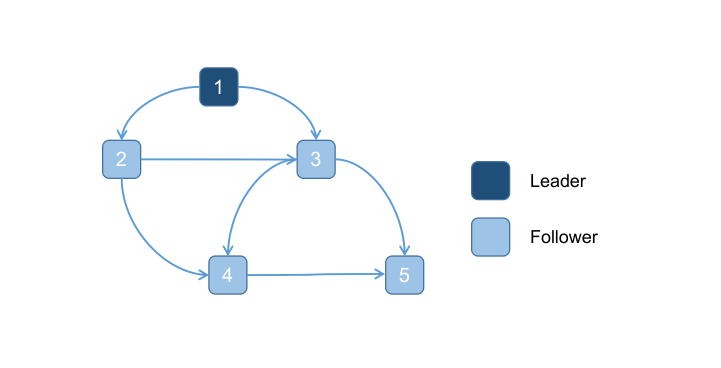
\includegraphics[width=0.6\textwidth]{formation.png}
	\caption{编队通信方法}
	\label{fig4-7}
\end{figure}

有$N_{2,1},N_{3,1},N_{3,2},N_{4,2},N_{4,3},N_{5,3},N_{5,4}$均不为0,则在这些对之间,按由小到大的顺序建立通信,传输长机的位置信息,保持相对位置的跟随。

在无人机发生编队队形变换时,则需要考虑最小总路径,可以用KM匈牙利算法解得每一架飞机对应的最小路径,并且在队形变换过程中需要考虑碰撞的影响。

图\ref{fig4-8}展示了三机编队的仿真结果:

\begin{figure}[!ht]
	\centering
	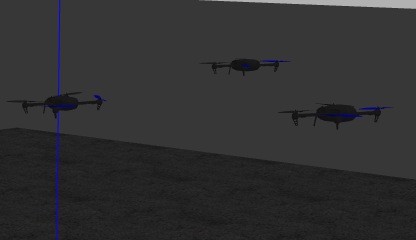
\includegraphics[width=0.5\textwidth]{multi.png}
	\caption{三机编队仿真}
	\label{fig4-8}
\end{figure}




\subsection{多机SLAM仿真} \label{4.3.3}

多机SLAM仿真除PX4的配置外,还要对SLAM的launch文件进行配置。其中包含了设置相机的参数文件,更重要的是配置各无人机所接受的相机话题。

\begin{lstlisting}[language={XML}]
<?xml version="1.0"?>
<launch>

<arg name="dist" default="0"/>
<arg name="cam" default="$(find ccmslam)/conf/px4_sitl.yaml"/>

<group ns="ccmslam">

<node pkg="tf" type="static_transform_publisher" name="linkC0_broadcaster" args="-100 300 5 -1.571 0 -2 world odomC0 100" /> 

<node pkg="ccmslam" type="ccmslamClientNode" name="ccmslamClientNode0" args="$(find ccmslam)/conf/ORBvoc.txt $(arg cam)" output="screen">

<!-- ++++++++++++++++++++++++++++++++++++++++++++++ -->
<!-- Agent Specific Params - !!!MUST BE ADJUSTED!!! -->

<param name="~FrameId" type="string" value="odomC0" />
<param name="~ClientId" type="int" value="0" />

<param name="~TopicNameCamSub" type="string" value="/iris0/usb_cam/image_raw" />

<param name="~MapInTopicName" type="string" value="MapOutServer0" unless="$(arg dist)" />
<param name="~MapInTopicName" type="string" value="MapOutServer0Disturbed" if="$(arg dist)" /> 

</node>

</group>
</launch>
\end{lstlisting}

启动时需要启动服务器和客户端,然后打开ORB-SLAM节点,最终结果如图:

\begin{figure}[!ht]
	\centering
	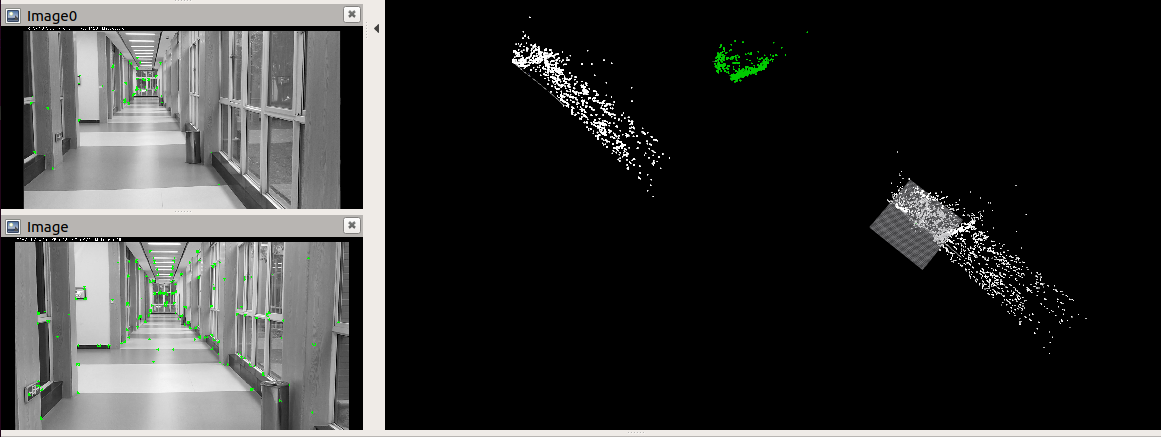
\includegraphics[width=0.9\textwidth]{ccm1.png}
	\caption{多机仿真结果}
	\label{fig4-9}
\end{figure}



































